\chapter{PROJETO E ARQUITETURA}\label{chap:projeto}

\section{Tema e escopo}

A aplicação representa um bate-papo no qual cada nó corresponde a um
participante. O escopo implementado prioriza o middleware: inicialização de
múltiplos processos, serialização das mensagens, comunicação ponto a ponto,
difusão ao grupo, registro das ordens local e global, relógio vetorial,
monitoramento, eleição e \textit{snapshot} distribuído. A interface é textual,
suficiente para observar os estados internos relevantes ao experimento.

O número de nós é informado em tempo de execução. O arquivo
\texttt{json/nodes.json} contém 15 entradas, e cada processo lê apenas as
primeiras $N$. Portanto, a configuração entregue suporta de 1 a 15 nós sem
alteração do código ou do arquivo de endereços, atendendo ao limite mínimo
solicitado pelo roteiro.

\section{Participação da equipe}

A divisão apresentada na Tabela~\ref{tab:equipe} foi construída a partir do
histórico de commits do repositório no \textit{GitHub}, mas as atividades de
integração, revisão, validação e criação do relatório foram conduzidas em
conjunto. Ademais, a partipação ativa do integrante, Lucas Carvalho de Borba,
no desenvolvimento foi reduzida devido a sua presença no evento \textit{LASC
    (Latin American Space Challenge)}.

\begin{table}[H]
    \centering
    \caption{Participação dos integrantes}
    \label{tab:equipe}
    \begin{tabular}{p{4.5cm} p{10.0cm}}
        \toprule
        \textbf{Integrante}     & \textbf{Principais contribuições}                \\
        \midrule
        Ian Callegari Aragão    & Configuração inicial; servidor e comunicação por
        sockets; tratamento de comandos; relógio vetorial; \text{health-check},
        estados dos nós e ajustes na eleição.                                      \\\\

        Lucas Losekann Rosa     & Interface de terminal e script de inicialização;
        mecanismo de ordenação e buffer de entrega; implementação e correções da
        eleição de líder; implementação do algorítimo de \textit{Chandy-Lamport}.  \\\\

        Lucas Carvalho de Borba & Testes na aplicação, validação dos requisitos e
        suporte na construção do relatório.                                        \\ \bottomrule
    \end{tabular}
\end{table}

\section{Tecnologias utilizadas}

A implementação foi escrita em Python 3.10 ou superior. O projeto é gerenciado
por \texttt{uv}, enquanto a comunicação, concorrência e serialização usam
principalmente módulos da biblioteca padrão: \texttt{socket},
\texttt{threading}, \texttt{json}, \texttt{dataclasses}, \texttt{argparse} e
\texttt{signal}. A rede é implementada diretamente sobre sockets TCP e a
interface usa sequências ANSI no terminal.

\section{Componentes da solução}

A Tabela~\ref{tab:componentes} relaciona as principais unidades do projeto.

\begin{table}[H]
    \centering
    \caption{Componentes do protótipo}
    \label{tab:componentes}
    \begin{tabular}{p{5.0 cm} p{10.0cm}}
        \toprule
        \textbf{Componente}           & \textbf{Responsabilidade}                          \\
        \midrule
        \texttt{lauch\_node.py}       & Lê os argumentos \texttt{--id} e
        \texttt{--count}, carrega o catálogo e instancia um nó.                            \\\\

        \texttt{services/node.py}     & Mantém relógios, históricos, buffer,
        sequências, estado dos pares, interface de comandos, heartbeat, eleição,
        recuperação da ordem e coordenação do snapshot.                                    \\\\

        \texttt{services/socket.py}   & Abre o servidor TCP, aceita conexões e envia
        documentos JSON.                                                                   \\\\

        \texttt{services/terminal.py} & Mantém uma área de rolagem e uma linha
        fixa de entrada para a interface textual.                                          \\\\

        \texttt{models/node\_dto.py}  & Define o formato lógico das mensagens.             \\\\

        \texttt{models/snapshot\_ses-}                                                     \\ \texttt{-sion.py} & Mantém os canais em gravação,
        estados de canal e relatórios de uma captura.                                      \\\\

        \texttt{json/nodes.json}      & Catálogo estático com IDs, endereço IP e portas.   \\\\

        \texttt{start.sh}             & Abre $N$ processos em terminais Konsole separados. \\\\

        \bottomrule
    \end{tabular}
\end{table}

Cada nó possui memória privada. Dentro do processo, três fluxos concorrentes
são iniciados: escuta TCP, emissão periódica de batimentos (\textit{heartbeat})
e verificação de saúde (\textit{health-check}). A interface é executada no
fluxo principal. Locks distintos protegem relógio vetorial, histórico local,
contador do sequenciador, entrega, heartbeat e eleição.

\begin{figure}[H]
    \centering
    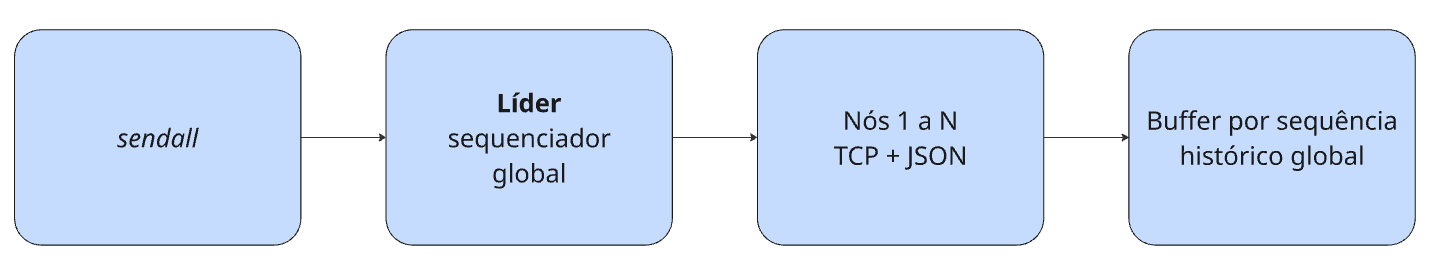
\includegraphics[width=1.0\textwidth]{04-figuras/fluxo_sendall.png}
    \caption{Fluxo de uma mensagem de grupo}
    \label{fig:arquitetura}
\end{figure}

\section{Formato e fluxo das mensagens}

As mensagens são serializadas como objetos JSON derivados de \texttt{NodeDto}.
Os campos comuns são: tipo, origem, horário, relógio vetorial e texto. Conforme
a operação, também são informados destino, sequência local e sequência global.
Os tipos declarados incluem mensagem privada, pedido de mensagem de grupo,
mensagem de grupo ordenada, heartbeat, confirmação de heartbeat, eleição,
coordenador, atualização da lista de nós, marcador e relatório de snapshot,
pedido e resposta de estado da ordem global. Os campos \texttt{channel\_origin}
e \texttt{channel\_sequence} identificam o emissor TCP e a posição da mensagem
no canal lógico sem confundi-lo com o autor original de uma mensagem
retransmitida pelo líder.

Em cada envio, \texttt{Socket.send} abre uma conexão TCP, transmite um
documento JSON e fecha a conexão. O receptor aceita a conexão, lê blocos de até
65.536 bytes até o fechamento do emissor e então delega o documento completo ao
nó \cite{python-socket}. A escolha por unicast TCP foi motivada pela entrega
confiável e pela simplicidade de endereçamento em uma única máquina. Para
difusão, o líder itera sobre o catálogo e envia uma cópia para cada
participante. Em comparação ao multicast UDP, essa solução evita implementar
confirmação e retransmissão de datagramas. 

Além disso, o multicast UDP não
oferece, por si só, um mecanismo específico para comunicação privada entre dois
participantes, sendo necessária a implementação de uma lógica adicional para
distinguir e encaminhar mensagens privadas. Com TCP unicast, essa distinção é
obtida naturalmente pelo endereço do destinatário da conexão, não sendo
necessário implementar um mecanismo adicional de comunicação privada. Como
contrapartida, a difusão realiza $N$ entregas por mensagem de grupo e concentra
esse custo no coordenador.

\section{Endereçamento}

Todos os ensaios foram executados pela interface de loopback, de modo que a
rede não sai da máquina local. Cada nó possui uma porta exclusiva, conforme a
Tabela~\ref{tab:enderecos}. O servidor escuta em \texttt{0.0.0.0}, enquanto o
catálogo usa \texttt{127.0.0.1} como destino.

\begin{table}[H]
    \centering
    \caption{Catálogo de endereços da simulação}
    \label{tab:enderecos}
    \setlength{\tabcolsep}{3pt}
    \small
    \begin{tabular}{ccc@{\hspace{0.6cm}}ccc@{\hspace{0.6cm}}ccc}
        \toprule
        \textbf{Nó} & \textbf{IP} & \textbf{Porta} &
        \textbf{Nó} & \textbf{IP} & \textbf{Porta} &
        \textbf{Nó} & \textbf{IP} & \textbf{Porta}                                                 \\
        \midrule
        1           & 127.0.0.1   & 5001           & 6  & 127.0.0.1 & 5006 & 11 & 127.0.0.1 & 5011 \\
        2           & 127.0.0.1   & 5002           & 7  & 127.0.0.1 & 5007 & 12 & 127.0.0.1 & 5012 \\
        3           & 127.0.0.1   & 5003           & 8  & 127.0.0.1 & 5008 & 13 & 127.0.0.1 & 5013 \\
        4           & 127.0.0.1   & 5004           & 9  & 127.0.0.1 & 5009 & 14 & 127.0.0.1 & 5014 \\
        5           & 127.0.0.1   & 5005           & 10 & 127.0.0.1 & 5010 & 15 & 127.0.0.1 & 5015 \\
        \bottomrule
    \end{tabular}
\end{table}

\section{Interface e execução}

O script automático depende de Linux, \texttt{bash}, \texttt{setsid},
\texttt{Konsole} e \texttt{uv}. Na raiz do repositório, a inicialização de
três, oito ou quinze nós é feita por:

\begin{lstlisting}[style=bash, numbers=none]
./start.sh --count <quantidade>
\end{lstlisting}

Também é possível abrir terminais manualmente e executar um processo em cada
um:

\begin{lstlisting}[style=bash, numbers=none]
uv run python lauch_node.py --id <identificador> --count <quantidade>
\end{lstlisting}

Os comandos da interface são descritos na Tabela~\ref{tab:comandos}.

\begin{table}[H]
    \centering
    \caption{Comandos disponíveis em cada nó}
    \label{tab:comandos}
    \begin{tabular}{p{4.5cm} p{9.5cm}}
        \toprule
        \textbf{Comando}              & \textbf{Função}                                          \\
        \midrule
        \texttt{send ID mensagem}     & Envia uma mensagem privada ao endereço do ID.            \\
        \texttt{sendall mensagem}     & Solicita ao líder a ordenação e difusão ao grupo.        \\
        \texttt{local}                & Exibe os envios produzidos localmente e sua sequência.   \\
        \texttt{global}               & Exibe as mensagens de grupo já entregues em ordem total. \\
        \texttt{status}               & Exibe líder, vetor, próxima sequência e históricos.      \\
        \texttt{list}                 & Exibe endereço e estado ativo/inativo dos participantes. \\
        \texttt{snapshot}             & Inicia \textit{Chandy-Lamport} e exibe o estado global após
        receber os fragmentos dos nós ativos.                                                    \\
        \texttt{help} & Lista os comandos disponíveis.                                            \\
        \texttt{exit} & Encerra o processo.                                                       \\
        \bottomrule
    \end{tabular}
\end{table}

No comando \texttt{send}, somente o emissor registra o evento em sua ordem
local. O documento \texttt{PRIVATE\_MESSAGE} é encaminhado ao endereço do
destino, que combina o vetor recebido com o seu relógio, incrementa a própria
posição e exibe a mensagem com o rótulo \texttt{[PRIVADA]}. Como se trata de
unicast, ela não recebe sequência global nem aparece no histórico dos demais
participantes.
